\chapter{Perkolation im Boolschen Modell}

Nun sollen die Perkolationseigenschaften eines por�sen Mediums untersucht werden. Als Modell f�r das por�se Medium wird das Boolsche Modell f�r die Perkolation verwendet. F�r die Untersuchung wird eine quadratische Simulationsbox mit der L�nge $L$ verwendet. In dieser Simulationsbox werden nun Kreise mit dem Radius $R=1$ verteilt, die die Hindernisse darstellen. Eine �berlappung der Kreise ist erlaubt. Man spricht von einem perkolierenden Cluster, wenn es eine durchg�ngige Fl�che von �berlappenden Kreisen gibt, die die gegen�berliegenden R�nder verbindet. Es l�sst sich zeigen, dass es ausreichend ist eine Perkolation in einer Richtung zu finden, um von allgemeiner Perkolation zu sprechen. W�re das System unendlich vergr��ert, bei gleichbleibender Dichte der Kreise, g�be es auch in der anderen Richtung eine Perkolation.

\begin{figure}[h!]
	\centering
		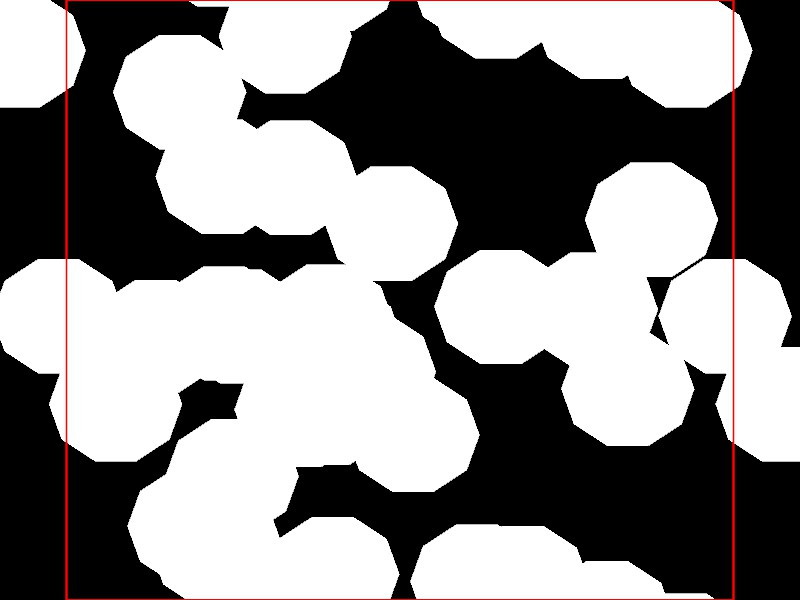
\includegraphics[width=0.80\textwidth]{img/perkolation.jpg}
	\caption{Beispiel eines perkolierenden Clusters. Die wei�e Fl�che stellt die �berlagernden Kreise da. Es ist m�glich, das System von oben nach unten auf der wei�en Fl�che zu durchqueren. Von rechts nach links gibt es kein perkolierendes Cluster. Aufgrund der periodischen Randbedingungen reicht allerdings eine Perkolation in eine Richtung. Im Unendlichen g�be es damit auch eine Perkolation in der Waagrechten.}
	\label{fig:perkolation}
\end{figure}

\begin{figure}[h!]
	\centering
		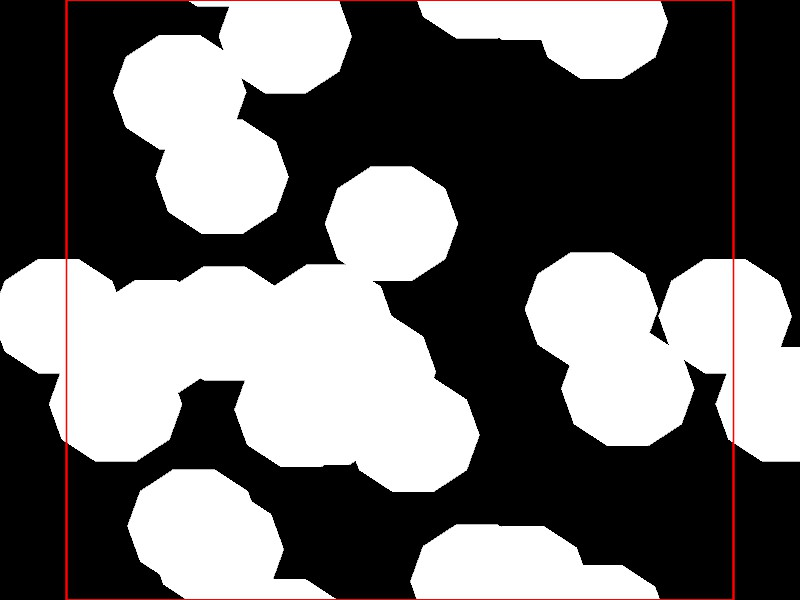
\includegraphics[width=0.80\textwidth]{img/nonperkolation.jpg}
	\caption{Beispiel f�r Cluster ohne Perkolation. Hier ist es weder m�glich, das Systen von rechts nach links noch von oben nach unten �ber die wei�e Fl�che zu durchschreiten.}
	\label{fig:nonperkolation}
\end{figure}



